\documentclass{article}
\usepackage{enumitem}
\usepackage{amsmath,amssymb,amsthm}
\usepackage{esvect}
\usepackage[a4paper, margin=1cm]{geometry}
\usepackage{stocktonmacros}
\usepackage{graphicx}
\graphicspath{ {./images/} }

\begin{document}
\begin{enumerate}
  \item Let $f(x)$ be a $2 \pi$-period function on the interval $[-\pi, \pi]$ where
  $\displaystyle
  f(x) =
  \begin{cases}
    -1 & - \pi < x \leq 0\\
    1 &\ \ 0 < x \leq \pi
  \end{cases}
  $
  % Personal addition - add the Fourier Series Formula
  \begin{align}
    a_n & = \frac{1}{L}  \int^L_{-L} f(x) \sin\left( \frac{n \pi x}{L} \right) \dx\\
    b_n & = \frac{1}{L}  \int^L_{-L} f(x) \cos\left( \frac{n \pi x}{L} \right) \dx\\
    b_0 & = \frac{1}{2L} \int^L_{-L} f(x) \dx
  \end{align}
  \begin{enumerate}
%______________________________________________________________________________%
%
% ans
    \item Plot the function on the interval $[-3\pi, 3\pi]$

    \begin{center}
      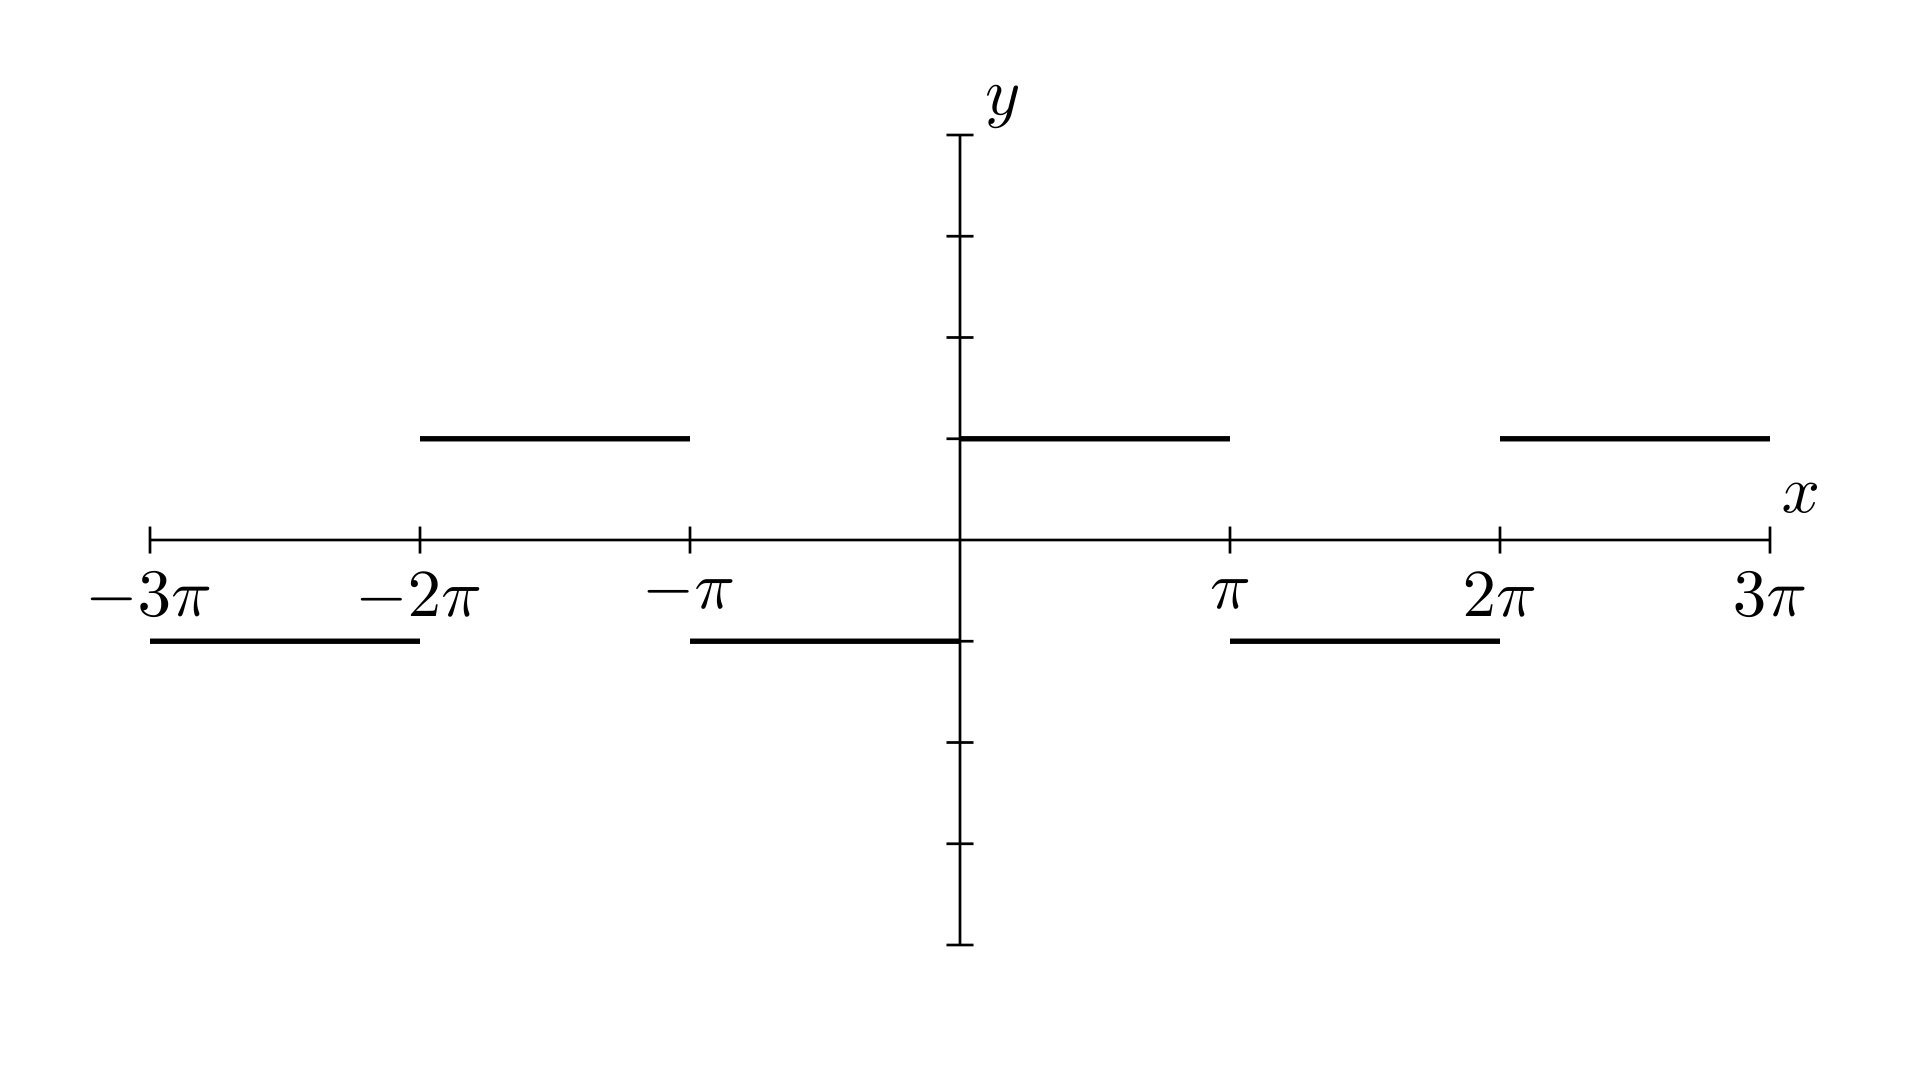
\includegraphics[height=10cm]{HomeworkiiProblemia}
    \end{center}
    \item Plot its (infinite) Fourier series on $[-3 \pi, 3 \pi]$

    \begin{center}
      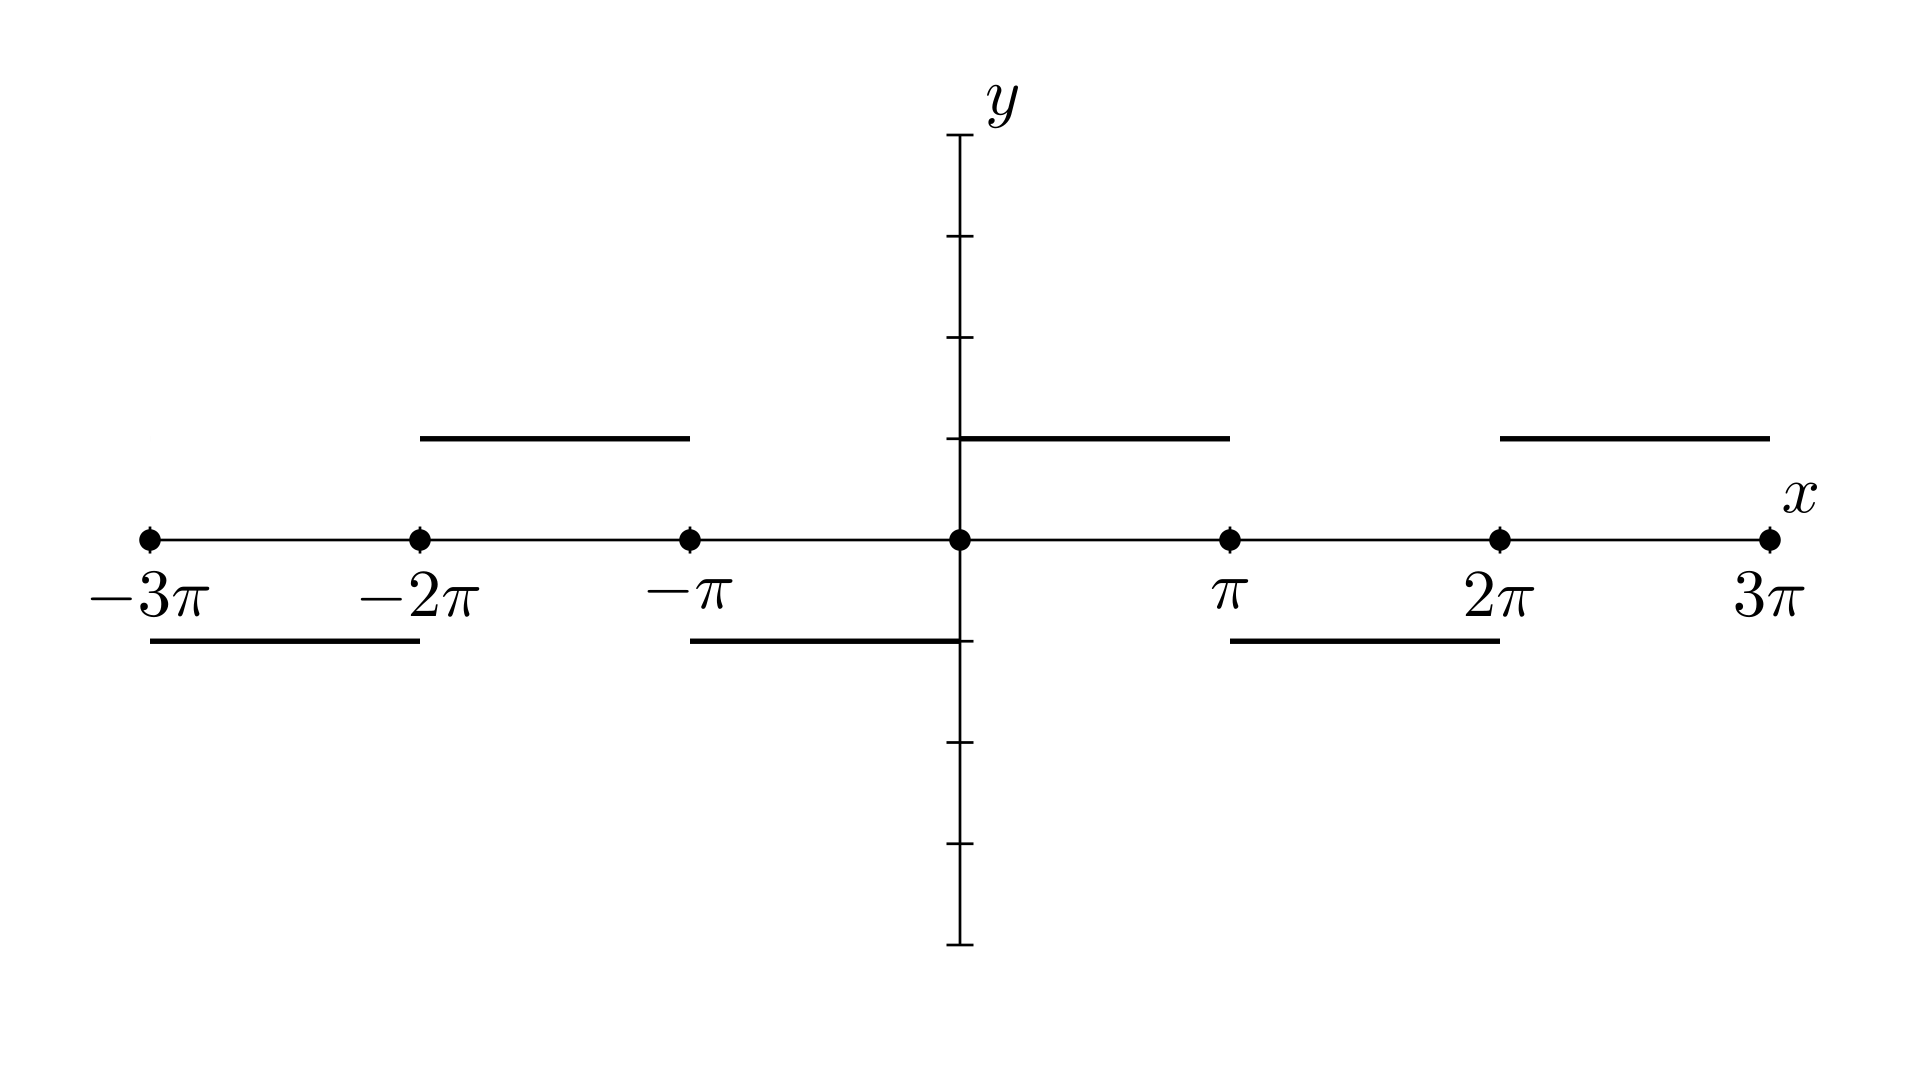
\includegraphics[height=10cm]{HomeworkiiProblemib}
    \end{center}
    \item Find the Fourier series of $f(x)$

    Here, let us consider the symmetry of our function.

    When we look at the graph of $f(x)$, we can see there is a reflection about the origin, making the function odd. $\sin$ is also an odd function, therefore $a_n$ is an even function.

    Looking at $b_n$, $\cos$ is an even function, therefore $b_n$ becomes an odd function.

    Finally, $b_0$ is always an odd function. When we integrate these three coefficients, we lose $b_n$ and $b_0$, but keep $a_n$. Since $a_n$ is even, we can write:
%
    \begin{align}
      a_n & = \frac{2}{L} \int^L_0 f(x) \sin\left( \frac{n \pi x}{L} \right) \dx
    \end{align}

    Here, we are looking at the interval from $0$ to $L$. Our given function, $f(x)$ runs from $-\pi$ to $\pi$, therefore our integral is:
%
    \begin{align}
      a_n & = \frac{2}{\pi} \int^\pi_0 1 \cdot \sin\left( \frac{n \pi x}{\pi} \right) \dx\\
      & = \frac{2}{\pi} \int^\pi_0 \sin\left( n x \right) \dx
    \end{align}

    From here, we can compute our integral:
    %
    \begin{align}
      a_n & = \frac{2}{\pi } \int^\pi_0 \sin\left( n x \right) \dx\\
      & = -\frac{2}{\pi n} \cos\left( n x \right) \bigg|^\pi_0\\
      & = \frac{2}{\pi n}\big( 1 - \cos( n \pi ) \big)
    \end{align}

    Here, we found our coefficient, $a_n$. Now, since $f(x)$ is odd, we are only interested in the following:
    %
    \begin{align}
      f(x) & = \sum^\infty_{n = 1} a_n \sin\left( \frac{n \pi x}{L} \right)\\
      & = \sum^\infty_{n = 1}
      \frac{2}{\pi n}\big( 1 - \cos( n \pi ) \big)
      \sin\left( \frac{n \pi x}{L} \right)
    \end{align}

    Here, since our interval is $-\pi$ to $\pi$, so let us write:
    %
    \begin{align}
      f(x) & =
      \sum^\infty_{n = 1}
      \frac{2}{\pi n}\big( 1 - \cos( n \pi ) \big)
      \sin\left( \frac{n \pi x}{\pi} \right)\\
      & =
      \sum^\infty_{n = 1}
      \frac{2}{\pi n}\big( 1 - \cos( n \pi ) \big)
      \sin\left( n x \right)
    \end{align}

    Here, we have our Fourier series.
%
%______________________________________________________________________________%
%
\newpage
\setcounter{equation}{0}
%
%______________________________________________________________________________%
%
\end{enumerate}
  \item Let $f(x) = x^2$ be a $2 \pi$-periodic function on the interval $[-\pi, \pi]$.
  \begin{enumerate}
    \item Derive its Fourier series
    %

    % ans
    Let us consider the symmetry of our function. Our function, $f(x)$, is an even function. Therefore, we have the following coefficients:
%
    \begin{align}
      b_n & = \frac{1}{L}  \int^L_{-L} f(x) \cos\left( \frac{n \pi x}{L} \right) \dx\\
      b_0 & = \frac{1}{2L} \int^L_{-L} f(x) \dx
    \end{align}

    Since $f(x)$ is even, we can write:
    %
    \begin{align}
      b_n & = \frac{2}{L}  \int^L_0 f(x) \cos\left( \frac{n \pi x}{L} \right) \dx\\
      b_0 & = \frac{1}{L} \int^L_0 f(x) \dx
    \end{align}

    In addition, since we also know our interval and our function, we can write:
    %
    \begin{align}
      b_n & = \frac{2}{\pi} \int^\pi_0 x^2 \cos\left( n x \right) \dx\\
      b_0 & = \frac{1}{\pi} \int^\pi_0 x^2 \dx
    \end{align}

    First, let us find the integral of $b_n$. Let us rewrite $b_n$ first:
    %
    \begin{align}
      b_n & = \frac{2}{\pi} \int^\pi_0 x^2 \cos\left( n x \right) \dx
    \end{align}

    Here, we want to do integration by parts. We want $x^2$ as our derived function since we can derive that function to $0$.

    \begin{center}
      \begin{tabular}{c|c}
        $x^2$ & $\displaystyle \cos(n x)$\\
        \hline
        $2x$ & $\displaystyle \frac{1}{n} \sin(n x)$\\
        \hline
        $2$ & $\displaystyle -\frac{1}{n^2} \cos(n x)$\\
        \hline
        $0$ & $\displaystyle -\frac{1}{n^3} \sin(n x)$
      \end{tabular}
    \end{center}

    Here, we can write our integral as the following:
    %
    \begin{align}
      b_n & = \frac{2}{\pi} \left[ \frac{x^2}{n} \sin(n x) + \frac{2x}{n^2} \cos(n x) - \frac{2}{n^3} \sin(n x) \right]^\pi_0\\
      & = \frac{2}{\pi n} \left[ x^2 \sin(n x) + \frac{2x}{n} \cos(n x) - \frac{2}{n^2} \sin(n x) \right]^\pi_0\\
      & = \frac{2}{\pi n} \left[ \pi^2 \sin(\pi x) + \frac{2\pi}{n} \cos(n \pi) - \frac{2}{n^2} \sin(n \pi) \right] - \frac{2}{n \pi} \left[ 0^2 \sin(0) + \frac{0}{n} \cos(0) - \frac{2}{n^2} \sin(0) \right]
    \end{align}

    Here, the entire right term zeroes out. On the left, $\sin(n \pi)$ zeroes out, leaving us with:
    %
    \begin{align}
      b_n & = \frac{4}{n^2} \cos(n \pi)
    \end{align}

    Now, let us find $b_0$:
    %
    \begin{align}
      b_0 & = \frac{1}{\pi} \int^\pi_0 x^2 \dx\\
      & = \frac{1}{\pi} \left[ \frac{x^3}{3} \right]^\pi_0\\
      & = \frac{1}{3\pi} \left[ x^3 \right]^\pi_0\\
      & = \frac{1}{3\pi} \left[ \pi^3 - 0 \right]\\
      & = \frac{\pi^2}{3}
    \end{align}

    Now that we have our coefficients, we can write:
    %
    \begin{align}
      f(x) & = \frac{\pi^2}{3} + \sum^\infty_{n = 1} \frac{4}{n^2} \cos(n \pi) \sin(n x)
    \end{align}
    %
    \item Use Maple of Matlab to plot its finite Fourier series on $[-\pi, \pi]$ for $N = 10, 20, 50$ together with $f(x)$
    %

    % ans

    %
    \item Use your Fourier series from part (a) to show that $\frac{\pi^2}{6} = 1 + \frac{1}{2^2} + \frac{1}{3^2} + \frac{1}{4^2} + \ldots$.
    %

    % ans
    Here, as we increase our $n$, our equation tends to flatten out to a straight line at around $y = 3.3$

    \begin{center}
      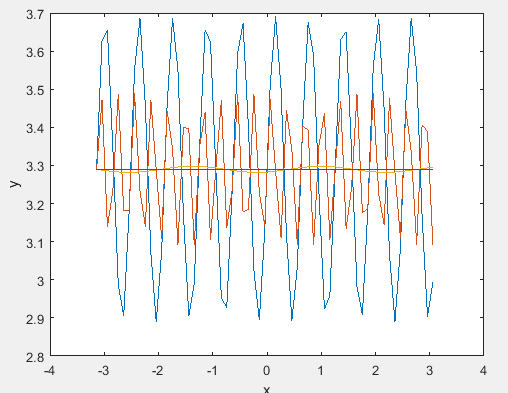
\includegraphics[height = 10cm]{Fourier}
    \end{center}

    %
  \end{enumerate}
%
%______________________________________________________________________________%
%
\newpage
\setcounter{equation}{0}
%
%______________________________________________________________________________%
%
  \item In the solution of the heat equation, we end up solving $X^{\prime\prime} = -\lambda X$. Show that if $\lambda < 0$ or $\lambda = 0$ there is only the trivial solution ($X(x) = 0$).

Here, we have the equation:
\begin{align}
  X^{\prime\prime} & = - \lambda X
\end{align}

We want to use this equation and set our boundary conditions as $X(0) = X(L) = 0$. Now, we must find an equation where after two derivatives on the right, we obtain a similar function on the left. On the left, we have a sign, coefficient, and function of $x$. Let us write a general solution for our equation:
%
\begin{align}
  X(x) & = A \cos(\sqrt \lambda x) + B \sin( \sqrt \lambda x)
\end{align}

Here, we can make three assumptions \ask{via trichotomy}: $\lambda < 0, \lambda = 0,$ or $\lambda > 0$. Let us look at the first two examples:

\begin{enumerate}
  \item $\lambda < 0$

  Here, let us consider the case when $\lambda$ is negative. Let us consider rewriting $\lambda$:
  %
  \begin{align}
    \lambda < 0\\
    \lambda \cdot -1 > 0 \cdot -1\\
    -1 \cdot \lambda > 0
  \end{align}

  Now, let us plug in our found value into our general equation:
  %
  \begin{align}
    X(x) & =
    A \cos (\sqrt{- 1 \cdot \lambda} x) +
    B \sin (\sqrt{- 1 \cdot \lambda} x)
  \end{align}

  Let us separate the terms under the radical:
%
  \begin{align}
    X(x) & =
    A \cos (\sqrt{- 1 \cdot \lambda} x) +
    B \sin (\sqrt{- 1 \cdot \lambda} x)\\
    & =
    A \cos (\sqrt{- 1} \sqrt{\lambda} x) +
    B \sin (\sqrt{- 1} \sqrt{\lambda} x)\\
    & =
    A \cos (i \sqrt{\lambda} x) +
    B \sin (i \sqrt{\lambda} x)
  \end{align}

  Here, in our expression, we see we are taking the square root of a negative number, which would give us an imaginary number. Here, we are evaluating our general solution with real numbers, therefore, the following form:
  %
  \begin{align}
    X(x) & =
    A \cos (i \sqrt{\lambda} x) +
    B \sin (i \sqrt{\lambda} x)
  \end{align}

  Where $X(x)$ is a real number would only have the trivial solution $X(x) = 0$.

  \item $\lambda = 0$

  Here, let us consider the case when $\lambda$ is zero. Now, let us write our general equation:
  %
  \begin{align}
    X(x) & = A \cos(\sqrt \lambda x) + B \sin(\sqrt \lambda x)
  \end{align}

  Here, since $\lambda = 0$, we can evaluate our equation:
  %
  \begin{align}
    X(x) & = A \cos(0) + B \sin(0)\\
    & = A
  \end{align}

  Now, let us evaluate our boundary condition for $X(x) = A$. First, we let $X(0) = 0$:
  %
  \begin{align}
    X(0) & = 0 = A
  \end{align}

  Here, we know $A$ is $0$. For the second condition, let us write:
  %
  \begin{align}
    X(L) & = 0 = A
  \end{align}

  Here, we will always have the trivial solution, $X(x) = 0$.

\end{enumerate}
%
%______________________________________________________________________________%
%
\newpage
\setcounter{equation}{0}
%
%______________________________________________________________________________%
%
  \item Show that $u(x, t) = e^{-\lambda^2 a^2 t}\left[ A \cos(\lambda x) + B \sin(\lambda x) \right]$




%______________________________________________________________________________%
%

% ans

Let us first consider the heat equation:
%
\begin{align}
  u_t & = \alpha^2 u_{xx}
\end{align}

Here, let us rewrite our equations:
%
\begin{align}
  XT^\prime & = \alpha^2 X^{\prime\prime}T\\
  \frac{T^\prime}{T} & = \alpha^2 \frac{X^{\prime\prime}}{X} = -\lambda
\end{align}

From here, we can see for the $T$, we will get an exponential whereas for the $X$ we will get a sine function. Let us rewrite $X$ first:
%
\begin{align}
  X(x) & = A \cos(\sqrt \lambda^2 x) + B \sin(\sqrt \lambda^2 x)\\
  X(x) & = A \cos(\lambda x) + B \sin(\lambda x)
\end{align}

Next, we rewrite $T$ as the following:
%
\begin{align}
  T(t) & = e^{-\lambda^2 \alpha^2 t}
\end{align}

We write $T$ in this form because when we derive $T$ once, we get a negative value, whereas when we derive it twice, we get a positive value. For $X$, we want to give it the general form in trig functions because after two derivatives, the equation looks similar but in the negative form.

Now, we assume our equation is seperable, therefore we can write:
%
\begin{align}
  T(t)X(x) & = e^{-\lambda^2 \alpha^2 t}[A \cos(\lambda x) + B \sin(\lambda x)]
\end{align}

%
%______________________________________________________________________________%
%
\bigbreak
\setcounter{equation}{0}
%
%______________________________________________________________________________%
%
  \item Solve $u_t = u_{xx}$ given $u(0, t) = u(1, t) = 0$ for $t \geq 0$ and $u(x, 0) = 1$ for $0 \leq x \leq 1$
%
%______________________________________________________________________________%
%

% ans
Let us consider the following conditions:
%
\begin{itemize}
  \item $u_t = u_{xx}$
  \item $u(0, t) = 0, t \geq 0$
  \item $u(1, t) = 0, t \geq 0$
  \item $u(x, 0) = 1, 0 \leq x \leq 1$
\end{itemize}

Let us begin finding our solution.
\begin{enumerate}
  \item Let us assume our solution is seperable. Therefore, we can write $u(x, t) = X(x)T(x)$. Now, using our initial conditions, let us write:
  %
  \begin{align}
    u(0, t) & = X(0)T(t) = 0 \Rightarrow X(0) = 0\\
    u(1, t) & = X(1)T(t) = 0 \Rightarrow X(1) = 0\\
    u(x, 0) & = X(x)T(0) = 0 \Rightarrow T(0) = 0
  \end{align}

  Now that we have used our initial conditions, let us write:
  %
  \begin{align}
    u_t & = u_{xx}\\
    XT^\prime & = X^{\prime\prime}T\\
    \frac{T^\prime}{T} & = \frac{X^{\prime\prime}}{X} = -\lambda
  \end{align}

  \item Here, we have more information regarding $X$, so let us write:
  %
  \begin{align}
    \frac{X^{\prime\prime}}{X} & = -\lambda\\
    X^{\prime\prime} & = -\lambda X
  \end{align}

  Here, we know $X(0) = X(1) = 0$. We want to write the general form of our equation as the following:
  %
  \begin{align}
    X(x) & = A \sin\left( \sqrt \lambda x\right) + B \cos\left( \sqrt \lambda x\right)
  \end{align}

  Here, we can input a condition for our general statement. Let us find $X(0)$ first:
  %
  \begin{align}
    X(0) = 0 & = A \sin(0) + B \cos(0)\\
    0 & = B\\
    X(x) & = A \sin(\sqrt \lambda x)
  \end{align}

  We also know $X(1) = 0$:
%
  \begin{align}
    X(1) = 0 & = A \sin(\sqrt \lambda)
  \end{align}

  Now, if $A$ is $0$, then our answer is trivial, therefore we want the inside of $\sin$ to be $n \pi$:
  %
  \begin{align}
    n \pi & = \sqrt \lambda\\
    n^2 \pi^2 & = \lambda_n
  \end{align}

  Therefore, we can write:
  %
  \begin{align}
    X_n(x) & = \sin(n \pi x)
  \end{align}

  \item Now, let us find $T$:
  %
  \begin{align}
    \frac{T^\prime}{T} & = -\lambda\\
    \frac{T^\prime}{T} & = - n \pi\\
    T^\prime_n & = - n \pi T\\
    T_n & = e^{-n \pi t}
  \end{align}

  \item Now, let us combine to find $u_n$
  %
  \begin{align}
    u_n(x, t) & = X_n(x)T_n(t)\\
    & = \sin(n \pi x) e^{-n \pi t}
  \end{align}

  By linearity,
  %
  \begin{align}
    u(x, t) & =
    % Summation
    \sum^\infty_{n = 1}
    % A term
    A_n
    % X_n
    \sin(n x \pi)
    % T_n
    e^{-n \pi t}
  \end{align}
  \item Here, we would use an initial condition to find $A_n$. We know $u(x, 0) = 1$, so let us write:
  %
  \begin{align}
    u(x, 0) & =
    % Summation
    \sum^\infty_{n = 1}
    % A term
    A_n
    % X_n
    \sin(n x \pi)
    % T_n
    = 1\\
    A_n & = 2 \int^1_0 \sin(n \pi x) \dx\\
    & = \frac{2}{n \pi} \left( -\cos(n \pi (1)) + \cos(0) \right)\\
    & = \frac{2}{n \pi} (-\cos(n \pi) + 1)
  \end{align}

  Here, let us write our formula as the following:
  %
  \begin{align}
    u(x, t) & = \sum^\infty_{n = 1} \frac{2}{n \pi}(-\cos(n \pi) + 1)\sin(n x \pi)
  \end{align}
\end{enumerate}

\newpage
%
%______________________________________________________________________________%
%
\item Find the solution to the previous problem if $u(x, 0) = x - x^2$ for $0 \leq x \leq 1$

% ans
\begin{itemize}
  \item $u_t = u_{xx}$
  \item $u(0, t) = 0, t \geq 0$
  \item $u(1, t) = 0, t \geq 0$
  \item $u(x, 0) = x - x^2, 0 \leq x \leq 1$
\end{itemize}

Here, by following the same steps as the previous problem, we would reach the same conclusion up to step $e$. At step $e$, we want to replace our condition with the fourth bullet:
%
\begin{align}
  u(x, 0) & = \sum^\infty_{n = 1} A_n \sin(n x \pi)e^{-n \pi t}
\end{align}

Simarly as the end of the last question,
%
\begin{align}
  A_n & = 2 \int^1_0 (x-x^2) \sin(n \pi x) \dx\\
  & = 2 \int^1_0 x\sin(n \pi x) - x^2\sin(n \pi x) \dx
\end{align}

Here, let us create two integration tables:

\begin{center}
  \begin{tabular}{c|c}
    $x$ & $\sin(n \pi x)$\\
    \hline
    $1$ & $- \frac{1}{n \pi} \cos(n \pi x) $\\
    \hline
    $0$ & $- \frac{1}{n^2\pi^2} \sin(n \pi x)$\\
    \\
  \end{tabular}
  \begin{tabular}{c|c}
    $x^2$ & $  \sin(n \pi x) $\\
    \hline
    $2x$  & $- \frac{1}{n\pi} \cos(n \pi x) $\\
    \hline
    $2$   & $- \frac{1}{n^2\pi^2} \sin(n \pi x) $\\
    \hline
    $0$   & $  \frac{1}{n^3\pi^3} \cos(n \pi x) $
  \end{tabular}
\end{center}

Here, let us apply our integration:
%
\begin{align}
  A_n & = 2
  \left(
  - \frac{x}{n \pi} \cos(n \pi x)
  + \frac{1}{n^2\pi^2} \sin(n \pi x)
  + \frac{x^2}{n \pi} \cos(n \pi x)
  - \frac{2x}{n^2\pi^2} \sin(n \pi x)
  - \frac{2}{n^3\pi^3} \cos(n \pi x)
  \right)^1_0\\
  & = 2\left(
  - \frac{1}{n \pi}    \cos(n \pi)
  + \frac{1}{n \pi}    \cos(n \pi)
  - \frac{2}{n^3\pi^3} \cos(n \pi)
  + \frac{2}{n^3\pi^3}
  \right)\\
  & = 4\left(
  - \frac{1}{n^3\pi^3} \cos(n \pi)
  + \frac{1}{n^3\pi^3}
  \right)\\
  & =
  \frac{4 - 4\cos(n \pi)}{n^3\pi^3}
\end{align}

Here, our equation is the following:
%
\begin{align}
  u(x, t) & = \sum^\infty_{n = 1} \frac{4 - 4\cos(n \pi)}{n^3\pi^3} \sin(n x \pi)e^{-n \pi t}
\end{align}
%

%
%______________________________________________________________________________%
%
\newpage
\setcounter{equation}{0}
%
%______________________________________________________________________________%
%
  \item Solve $u_t = u_{xx}$ given $u(0, t) = u(1, t) = 0$ for $t \geq 0$ and $u(x, 0) = 10^{-5} \sin(10^6 \pi x)$ for $0 \leq x \leq 1$. Determine $u(x, 2)$ and $u(x, -2)$ and look at their magnitudes. Note that when $t = -2$, we are looking at the backward heat equation and given the magnitude of $u(x, -2)$, what can you say about the solution to the backward heat equation?

  % ans
  Let us consider the following conditions:
  \begin{itemize}
    \item $u_t = u_{xx}$
    \item $u(0, t) = 0, t \geq 0$
    \item $u(1, t) = 0, t \geq 0$
    \item $u(x, 0) = 10^{-5} \sin(10^6 \pi x), 0 \leq x \leq 1$
    \item Determine the following and look at their magnitudes
    \begin{itemize}
      \item $u(x, 2)$
      \item $u(x, -2)$
    \end{itemize}
  \end{itemize}

  Now, let us begin:

  \begin{enumerate}
    \item First, let us assume our equation is separable:
    %
    \begin{align}
      X(x)T^\prime(t) & = X^{\prime\prime}T(t)
    \end{align}

    Using our boundary conditions, we can find the following:
    %
    \begin{align}
      u(0, t) & = 0 = X(0)T(t) \Rightarrow X(0) = 0\\
      u(1, t) & = 0 = X(1)T(t) \Rightarrow X(1) = 0
    \end{align}

    Now, let us separate:
    %
    \begin{align}
      u_t & = u_{xx}\\
      XT^\prime & = X^{\prime\prime}T\\
      \frac{T^\prime}{T} & = \frac{X^{\prime\prime}}{X} = -\lambda
    \end{align}

    \item Here, let us solve for $X$:
    %
    \begin{align}
      X(x) & = A \sin( \sqrt \lambda x) + B \cos( \sqrt \lambda x)\\
      X(0) = 0 & = B\\
      X(1) = 0 & = A \sin( \sqrt \lambda )\\
      n \pi & = \sqrt \lambda\\
      n^2 \pi^2 & = \lambda\\
      X_n(x) & = \sin(n \pi x)
    \end{align}

    \item Now, let us solve for $T$:
    %
    \begin{align}
      \frac{T^\prime}{T} & = - n^2 \pi^2\\
      T^\prime & = - n^2 \pi^2 T_n\\
      T_n & = e^{-n^2 \pi^2 t}
    \end{align}

    \item Now, let us combine both $T_n$ and $X_n$:
    %
    \begin{align}
      u_n(x, t) & = X_n(x)T_n(x)\\
      & = \sin(n \pi x) e^{-n^2 \pi^2 t}
    \end{align}

    By linearity,
    %
    \begin{align}
      u(x, t) & =
      % sum
      \sum^\infty_{n = 1}
      % A_n
      A_n
      % X_n
      \sin(n \pi x)
      % T_n
      e^{-n^2 \pi^2 t}
    \end{align}

  \item Here, let us use our initial condition to find $A_n$:
  %
  \begin{align}
    2 \int^1_0 10^{-5}\sin(10^6 \pi x) \sin(n \pi x) \dx
  \end{align}

  Here, we can find our $A_{10^6}$ with the help of our initial condition. We know at $n= 10^6$ that $A_{10^6} = 10^{-5}$, so let us write:
  \begin{align}
    u(x, t) & = 10^{-5} \sin(10^6 \pi x)e^{-(10^6)^2 \pi^2 t}\\
    u(x, t) & = 10^{-5} \sin(10^6 \pi x)e^{-10^{12} \pi^2 t}
  \end{align}

  Here, using our equation, let us set $t$ to both $2$ and $-2$:
  \begin{align}
    u(x, 2) & = 10^{-5} \sin(10^6 \pi x)e^{-10^{12} \pi^2 2}\\
    & = \frac{\sin(10^6 \pi x)}{10^5 e^{10^{12} \pi^2 2}}\\
    u(x, -2) & = 10^{-5} \sin(10^6 \pi x)e^{-10^{12} \pi^2 (-2)}\\
    & = \frac{\sin(10^6 \pi x) e^{10^{12} \pi^2 2}}{10^5}
  \end{align}

  Here, our magnitudes from the origin changes drastically. Whereas at $t = 2$ tends to stay close to $0$ for a while, $t = -2$ blows up drastically.
\end{enumerate}
%%%

\end{enumerate}




\end{document}
